La misura della velocità della luce ha un interesse fisico molto elevato in quanto rappresenta uno dei valori notevoli con importantissime ripercussioni concrete nella realtà in cui viviamo. Uno dei primi tentativi concreti di misurare la velocità della luce è stato effettuato durante il XVI secolo da Galileo Galilei, che sospettava che la luce non si propagasse istantaneamente. Altri tentativi vennero svolti durante il XVII e XVIII secolo da Olaus Roamer attraverso osservazioni  astronomiche.\\

La difficoltà di questa misura risiede negli ordini di grandezza:  se si vuole misurare la velocità della luce a partire dalla formulazione classica (spazio percorso diviso al tempo necessario per percorrerlo) si incontrano svariati problemi originati dagli enormi spazi richiesti e dai piccolissimi tempi ottenuti. Per riuscire a misurare più agevolmente la velocità della luce serve dunque trovare un fenomeno alternativo che dipenda da tale grandezza ma che sia facilmente misurabile e non richieda apparati strumentali eccessivamente grandi. Così nel 1849, Hippolyte Fizeau sviluppò un nuovo metodo, successivamente modificato da Foucault.\\

Il metodo di Fizeau era basato su una ruota dentata, in grado di ruotare a velocità angolare decisa dallo sperimentatore, sul cui bordo veniva mandato un raggio luminoso (in modo che questo venisse bloccato o meno in presenza o assenza di un dente della ruota). Ponendo uno specchio piano distante dalla ruota, affinché il raggio venisse riflettuto e tornasse indietro percorrendo il medesimo tragitto dell'andata, ci si rende conto che l'intensità luminosa che ritorna al punto della sorgente è minima a velocità angolari della ruota ben precise, che corrispondono alle velocità angolare necessaria affinché un dente della ruota occupi lo spazio occupato da un buco nel tempo in cui la luce compie il percorso di andata e di ritorno. A partire da tali valori di velocità angolare, è possibile calcolare la velocità della luce.\\

Il problema legato al metodo di Fizeau deriva dal fatto che pur utilizzando un fascio di luce molto collimato come può essere la luce prodotta da un laser, a grande distanza (nell'ordine di $10\,km$) diverge. Un'altra complicazione consiste nel posizionare lo specchio in modo tale che sia perfettamente allineato e che faccia tornare il fascio di luce esattamente da dove è arrivato. o anche semplicemente dalla non omogeneità dello spazio percorso dalla luce in quanto può cambiare l'indice di rifrazione.
%Parola importante è collimare e sapere bene cosa è un collimatore (detto dalla prof a lezione)
Nel 1850 fu introdotto il metodo di Foucault, adottato in laboratorio, in cui viene completamente rimossa la ghiera rotante e vengono introdotti uno specchio concavo e uno specchio rotante.
\begin{figure}[htp!]
  \centering
  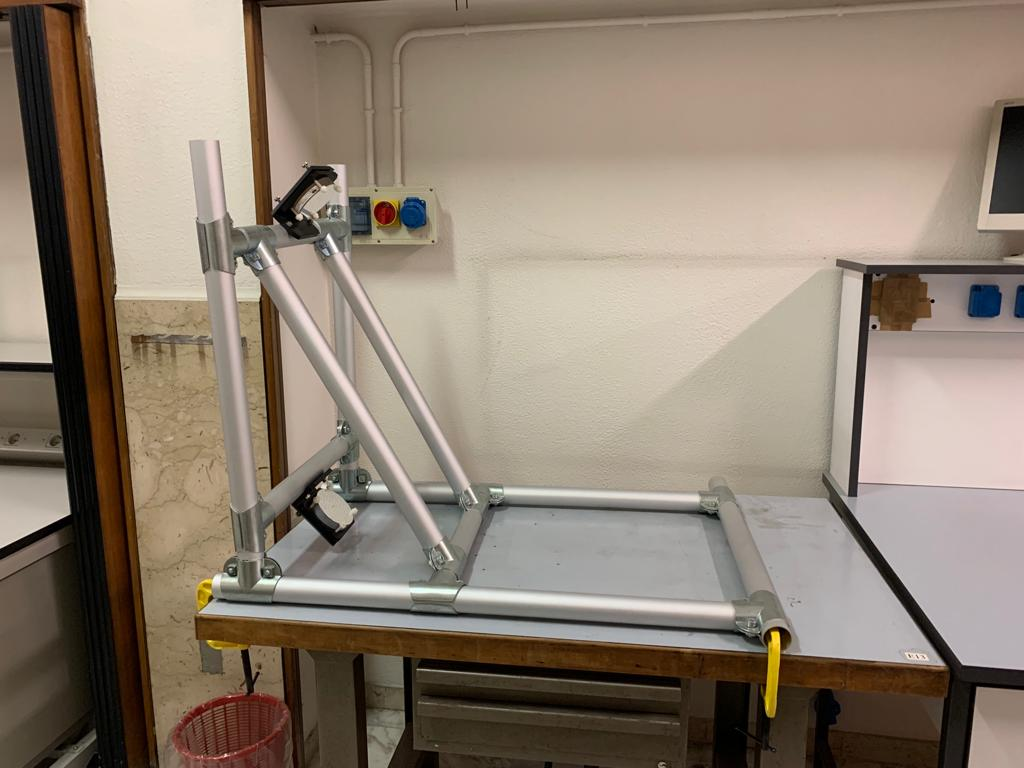
\includegraphics[scale=0.18]{Immagini/2.jpeg} 
  \centering
  \qquad 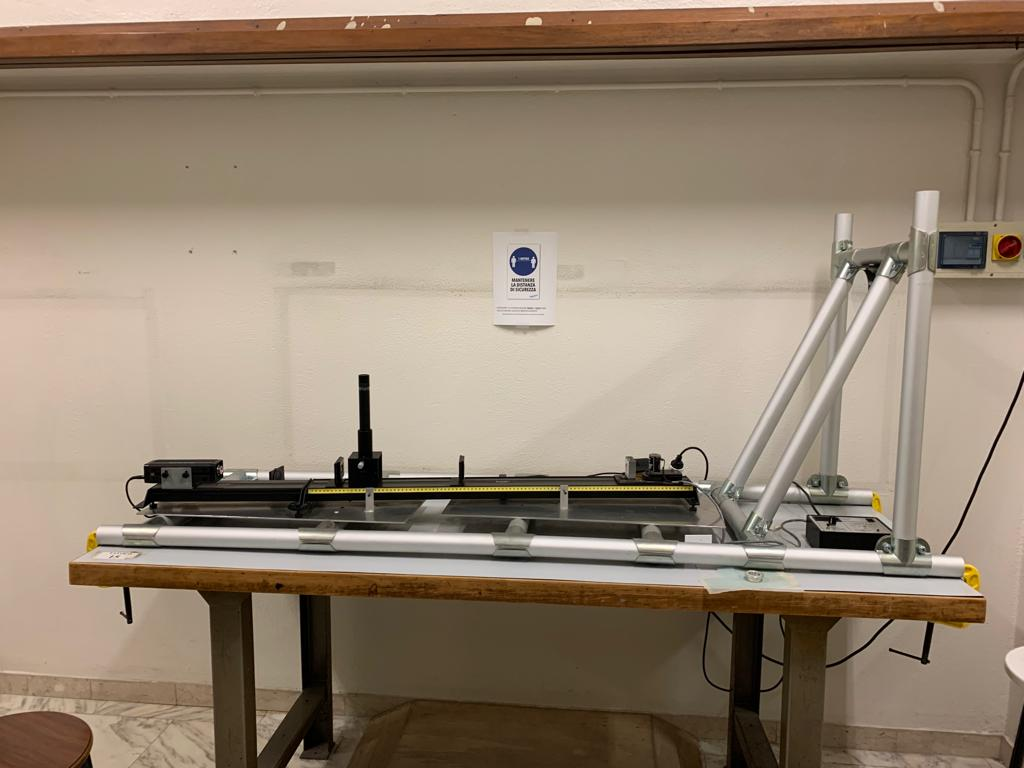
\includegraphics[scale=0.18]{Immagini/1.jpeg}
  \caption{Nelle due immagini si può osservare sistema sperimentale presente in laboratorio. Nella prima foto sono presenti i due specchi piani mentre a destra (posti ad una distanza considerevole) è presente l'apparato principale composto dal laser, ottiche, specchio concavo e rotante.}
\end{figure}